%% ============================================================
%%  A learned peak finder for VFE/LVR board QC current traces
%%  Full write-up: toy study, real traces, comparison with the existing finder
%%  Build (from writeup/src): pdflatex twice. Figures: python -m writeup.make_figures
%% ============================================================
\documentclass[11pt,a4paper]{article}
\usepackage[margin=2.3cm,bottom=2.8cm]{geometry}
\usepackage[T1]{fontenc}
\usepackage{lmodern}
\usepackage{amsmath,amssymb}
\usepackage{graphicx}
\usepackage{booktabs}
\usepackage{caption}
\usepackage{fancyhdr}
\usepackage[section]{placeins}
\usepackage{xcolor}
\usepackage{hyperref}
\hypersetup{colorlinks=true,linkcolor=blue!50!black,urlcolor=blue!50!black}
\captionsetup{font=small,labelfont=bf}
\graphicspath{{../plots/}}
\input{../plots/real/numbers.tex}

\newcommand{\us}{\,\textmu s}
\newcommand{\unsigned}{Unsigned algorithm steps (not yet signed off): dataset build and the inrush (P0) rule;
  run-level split; network training; peak read-out (argmax per output channel on 10\us\ bins; also the sub-bin read-out).}

\pagestyle{fancy}
\fancyhf{}
\renewcommand{\headrulewidth}{0pt}
\fancyfoot[R]{\thepage}
\fancyfoot[L]{\parbox[b]{0.9\textwidth}{\tiny\color{black!60}\unsigned}}
\fancypagestyle{plain}{\fancyhf{}\fancyfoot[R]{\thepage}%
  \fancyfoot[L]{\parbox[b]{0.9\textwidth}{\tiny\color{black!60}\unsigned}}}
\setlength{\footskip}{30pt}

\title{A learned peak finder for VFE/LVR board quality-control traces\\[4pt]
  \large From a toy study to real tester data, compared with the existing finder}
\author{Santanu Mahata}
\date{11 November 2026}

\begin{document}
\maketitle

\begin{abstract}
Board quality control reads five landmarks, P0--P4, off a current trace recorded for every shot. A
hard-coded finder does this today and on some shots reports three peaks instead of four. I train a 1D
convolutional network that outputs one heat-map per landmark and reads each position as the maximum of
its channel, with the height of that maximum as a per-landmark confidence. I first develop it on simulated
traces, then train it on \NShots\ shots from \NRuns\ four-peak runs of the LVR tester, with the existing
finder's times as labels. On \NVal\ shots from \NValRuns\ runs never used in training, the network agrees
with the finder to a median of \MedUnet\us; all four peaks lie within 0.02\,ms of the finder on \TwoUnet\%
of shots and within 0.1\,ms on \TenUnet\%. On the \NFail\ shots where the finder reported only three
peaks, the network places all five landmarks. Four steps of the real-data chain are not yet signed off;
they are named at the foot of every page.
\end{abstract}

\tableofcontents
\newpage

%% ------------------------------------------------------------
\section{Introduction}

Each VFE/LVR board under test is powered up repeatedly, and for every shot the tester records the input
current on scope channel C4. Five landmarks are read off that trace: the inrush spike, which I call P0,
and four peaks that the existing finder names A1, B1, A2 and B2. I call those four P1--P4, in time order.

The existing finder is hard-coded: fixed thresholds and windows. On some shots it misidentifies the
peaks, and each such shot needs a person to look at the trace. In the tester archive used here it
reported three peaks instead of four on \NFail\ shots (Section~\ref{sec:failures}).

My aim is a finder that learns the landmark positions from labelled traces instead of hand-tuned
thresholds, and that reports a confidence for each landmark, so that doubtful shots can be flagged
automatically. This note describes the method (Section~\ref{sec:method}), the toy study I used to develop
it before real traces were available (Section~\ref{sec:toy}), the real data and how I built a training set
from it (Section~\ref{sec:data}), training on real traces (Section~\ref{sec:training}), the comparison with
the existing finder (Sections~\ref{sec:results} and~\ref{sec:failures}), a study of model size and training
seed (Section~\ref{sec:sweep}), and what is still open (Section~\ref{sec:status}).

%% ------------------------------------------------------------
\section{Method}
\label{sec:method}

\paragraph{Heat-map formulation.}
The network reads the whole trace, $x \in \mathbb{R}^{n}$, and emits five output channels of the same
length, one per landmark. Channel $k$ is trained against a Gaussian target centred on the labelled
position $p_k$,
\begin{equation}
  y_k(t) = \exp\!\left[-\tfrac{1}{2}\,\frac{(t-p_k)^2}{\sigma^2}\right],
\end{equation}
with the per-sample binary cross-entropy between $\mathrm{sigmoid}(z_k(t))$ and $y_k(t)$ as loss, where
$z_k$ is the network's logit. The target width is $\sigma = 4$ samples on the toys and
$\sigma = \SigmaBins$ bins (30\us) on real traces.

\paragraph{Read-out and confidence.}
The reported position of landmark $k$ is $\hat p_k = \arg\max_t \mathrm{sigmoid}(z_k(t))$, and its
confidence is the value at that maximum, $c_k = \max_t \mathrm{sigmoid}(z_k(t)) \in [0,1]$. The channels
are separate, so each one only has to find its own landmark. As an option, a sub-bin position is read by
fitting a parabola through the highest bin and its two neighbours, with the offset clipped to $\pm 1$ bin:
\begin{equation}
  \hat p_k^{\,\mathrm{sub}} = \hat p_k + \frac{1}{2}\,\frac{s_{-}-s_{+}}{s_{-}-2s_0+s_{+}},
\end{equation}
where $s_0$ is the channel at $\hat p_k$ and $s_\pm$ its neighbours.

\paragraph{Input normalisation.}
Every trace is scaled on its own before it enters the network: subtract the median, then divide by the
largest absolute value. Absolute gain therefore does not enter. Any inference path must repeat this step
exactly; it is part of the model.

\paragraph{Network.}
The baseline is a 1D U-Net: each level is two convolutions of kernel width 9, each followed by batch
normalisation and ReLU; max-pooling by 2 on the way down, transposed convolutions on the way up, and skip
connections between matching levels. A $1\times1$ convolution maps the last decoder level to the five
logit channels. With base width 16 and three levels it has 0.46\,M parameters. For the real traces I also
use a configurable version (base width $b$, $L$ levels, channel count doubling per level up to 512); the
report model is $b=32$, $L=4$ with \ParamsUnet\,M parameters (Section~\ref{sec:sweep} explains the
choice). As a comparison I train a transformer: a convolutional stem, patches of 16 bins embedded as
tokens with a learned position code, a stack of self-attention encoder layers, and a transposed
convolution back to full resolution fused with the stem's features.

\paragraph{Why not regress five numbers.}
A network that regresses the five positions directly gives no per-landmark confidence, which is the part
quality control needs. I did not pursue it.

%% ------------------------------------------------------------
\section{Toy study}
\label{sec:toy}

Before real traces were available I developed the method on simulated traces, written from a verbal
description of the waveform. The numbers in this section are measured on simulation and are a check of
the method, not a result about boards.

\subsection{Generator}
A toy trace has 1024 samples (Figure~\ref{fig:anatomy}). A train of small spikes ends in P0, the last of them; P1 follows 10--60 samples later. P1--P4 rise in height within a trace, and after
each one the floor settles higher than before. Small decoy bumps ride on those floors. Rise and decay
widths are drawn independently. Table~\ref{tab:toygen} lists every range; all of them are guesses from the
description. Labels sit on the visible apex of the noiseless waveform; draws in which a landmark has no
visible apex are redrawn.

\begin{figure}[!htbp]
  \centering
  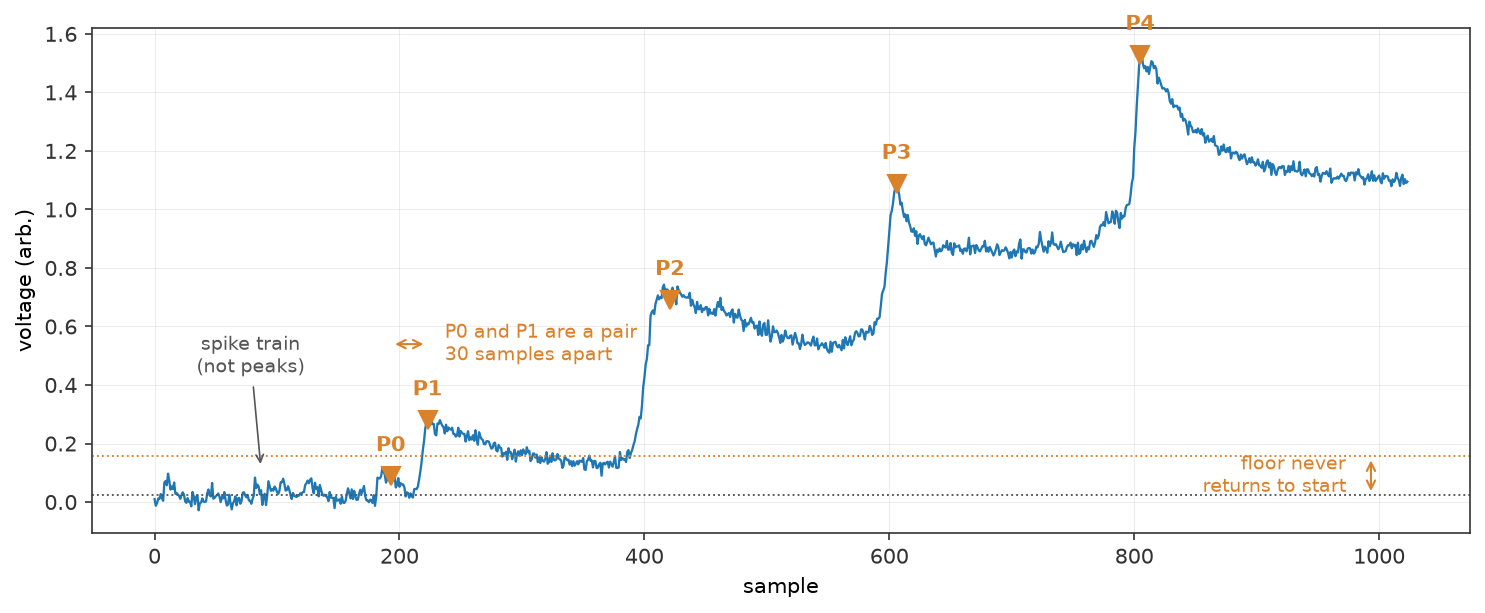
\includegraphics[width=0.9\textwidth]{toy/anatomy.png}
  \caption{One simulated trace. Markers are the five true landmark positions. Amplitude in arbitrary
  units; shape only.}
  \label{fig:anatomy}
\end{figure}

\begin{table}[!htbp]
  \centering\small
  \caption{Toy generator settings (\texttt{src/toy\_waveforms.py}, \texttt{ToyConfig}).}
  \label{tab:toygen}
  \begin{tabular}{@{}ll@{}}
    \toprule
    ingredient & range used \\
    \midrule
    trace length & 1024 samples \\
    P1--P4 live in & samples 143--922 \\
    P0 apex ahead of P1 apex by & 10--60 samples \\
    spikes before P0 & 8--20, height 0.01--0.06 \\
    P0 height & 0.04--0.09 \\
    P1--P4 heights & 0.25--1.00, increasing within a trace \\
    leading-edge width & 1.5--14 samples \\
    trailing decay & 2.5--30 samples, drawn independently \\
    per-trace shape tilt & 0.5--2.0 \\
    fraction of a peak left as floor & 0.25--0.55 \\
    floor step width & 3--10 samples \\
    decoy bumps per floor & 2--6, at 4--18\% of the local step \\
    noise & 0.004--0.015, plus 0.2\% single-sample glitches \\
    landmark spacing jitter & 50\% of the mean spacing \\
    \bottomrule
  \end{tabular}
\end{table}

\begin{figure}[!htbp]
  \centering
  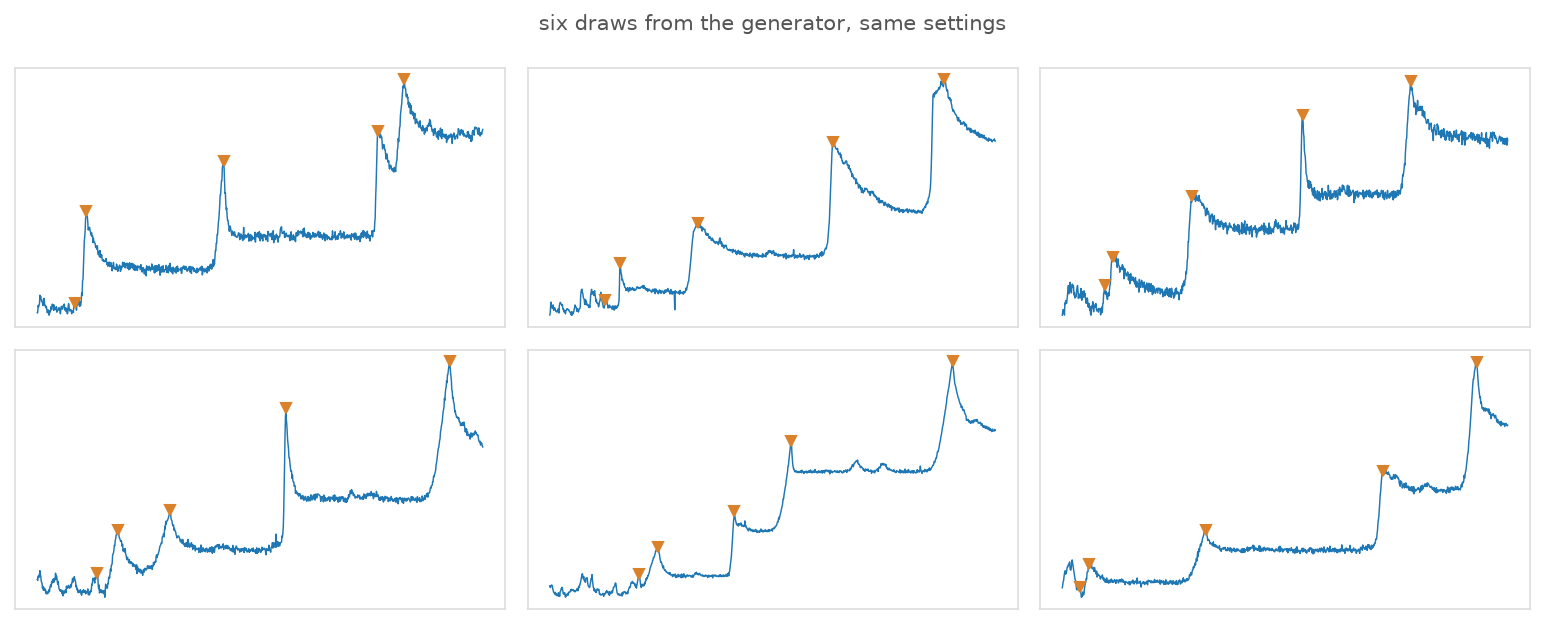
\includegraphics[width=0.95\textwidth]{toy/gallery.png}
  \caption{Six independent draws with the same generator settings. Each panel is scaled on its own.}
  \label{fig:gallery}
\end{figure}

\subsection{Training and results}
I trained the 0.46\,M-parameter U-Net on 8000 simulated traces for 25 epochs (Adam, learning rate
$10^{-3}$ with cosine decay, batch 32; 125\,s on one GPU) and tested it on 1000 held-out traces.
Figure~\ref{fig:heatmap} shows one held-out trace with the five channel outputs. All five landmarks fall
within 2 samples of the truth on 76.8\% of traces and within 4 samples on 89.0\%; at least one is more
than 15 samples off on 2.0\%. Figure~\ref{fig:perpeak} breaks this down by landmark.

\begin{figure}[!htbp]
  \centering
  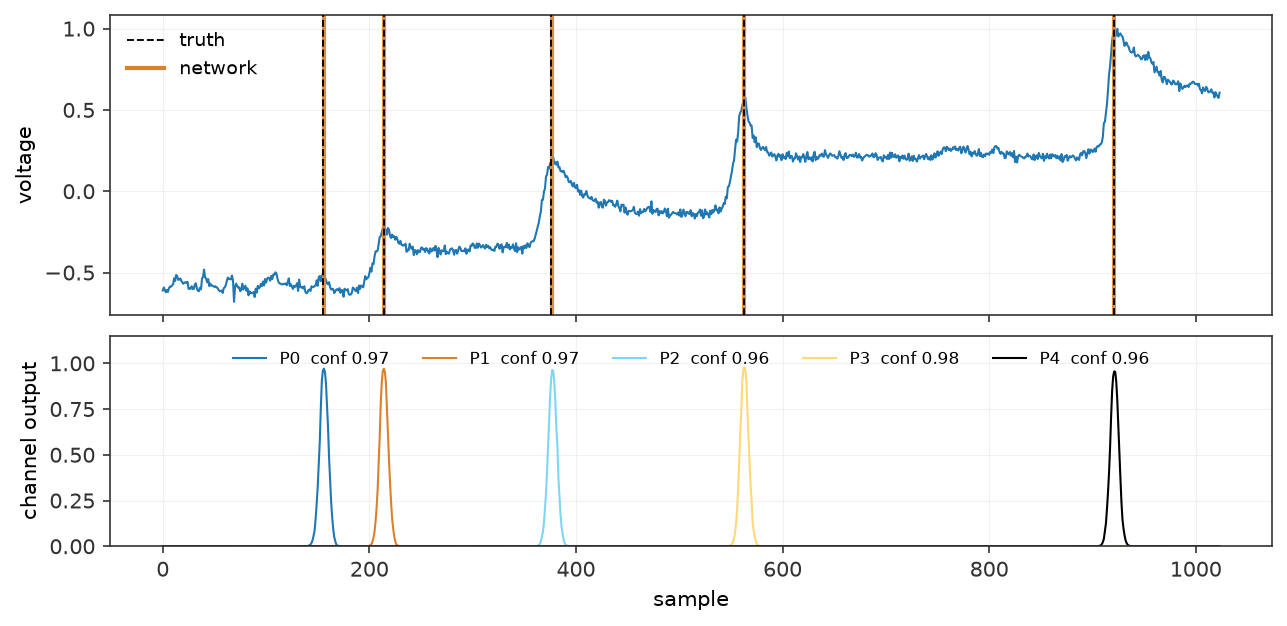
\includegraphics[width=0.9\textwidth]{toy/heatmap_demo.png}
  \caption{Top: a held-out simulated trace, true positions dashed, network positions solid. Bottom: the
  five channel outputs, with the confidence each one reaches.}
  \label{fig:heatmap}
\end{figure}

\begin{figure}[!htbp]
  \centering
  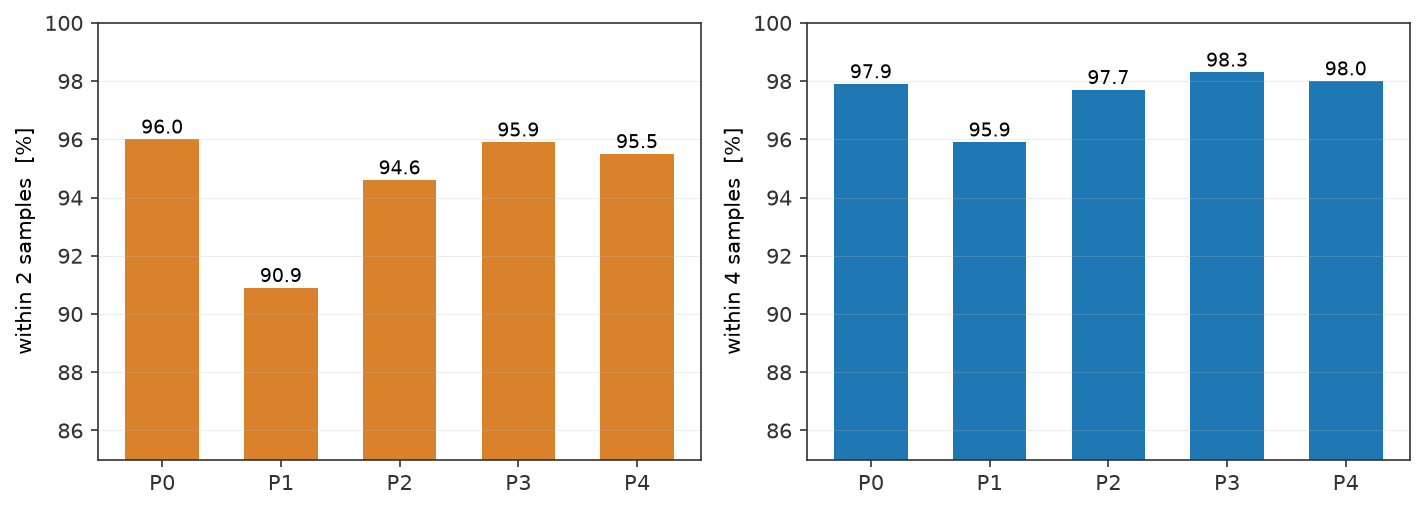
\includegraphics[width=0.85\textwidth]{toy/perpeak.png}
  \caption{1000 held-out simulated traces: fraction where each landmark lies within 2 (left) and 4 (right)
  samples of the visible apex. Suppressed zero.}
  \label{fig:perpeak}
\end{figure}

The misses are mostly 3 samples, just over the 2-sample line. P0 misses on 40 traces, 8 of them by more
than 15 samples; about half land earlier, in the spike train, and none on P1
(Figure~\ref{fig:p0errors}).

\begin{figure}[!htbp]
  \centering
  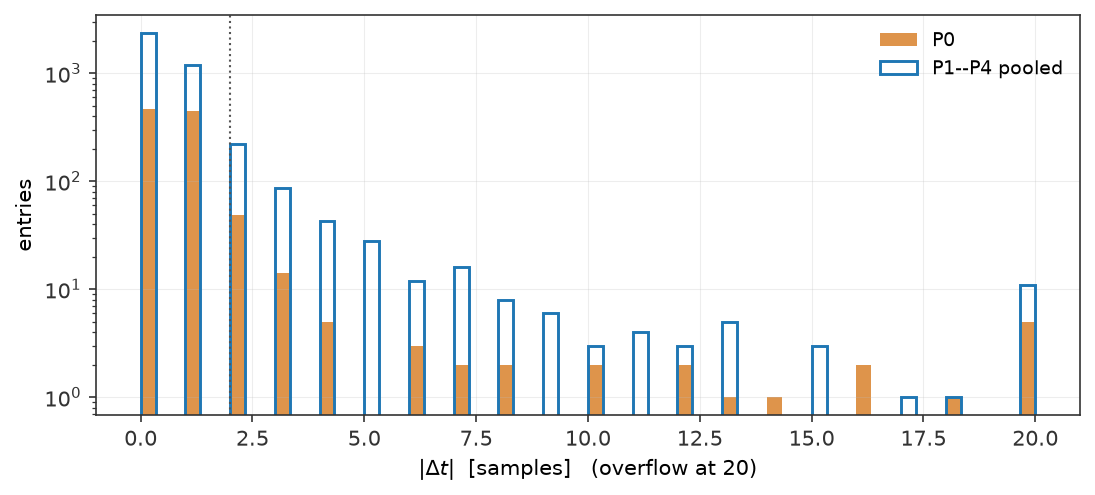
\includegraphics[width=0.7\textwidth]{toy/p0_errors.png}
  \caption{Absolute error on held-out simulated traces: P0 (1000 entries, filled) against P1--P4 pooled
  (4000 entries, outline). Log scale; dotted line at 2 samples; overflow in the last bin.}
  \label{fig:p0errors}
\end{figure}

\subsection{How precisely can an apex be located?}
I checked whether the 2-sample criterion is reachable on these traces at all. Readers that are told where
each peak is and take the highest sample nearby reach a lower all-five-within-2 fraction than the network
(Figure~\ref{fig:precision}, left). On 74\% of traces at least one apex has another sample within one noise
$\sigma$ of its height three or more samples away, so on these traces an apex is known to about 3 samples.
This is not a strict bound: a reader that knows the pulse shape could average over more samples. Narrower
targets, longer training and more training data did not move the network's number up
(Figure~\ref{fig:precision}, right).

\begin{figure}[!htbp]
  \centering
  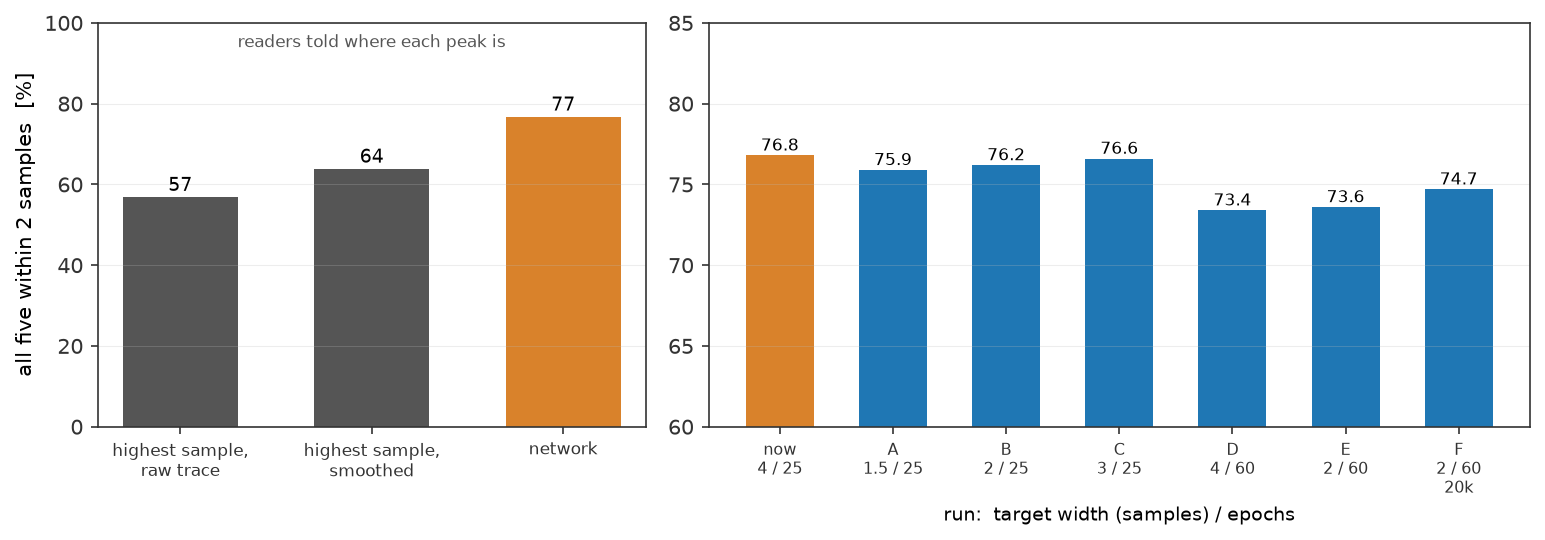
\includegraphics[width=0.95\textwidth]{toy/precision.png}
  \caption{Left: readers told where each peak is, taking the highest sample of the raw or smoothed trace,
  against the network. Right: the network retrained with different target widths and epochs (one run uses
  20\,k training traces). 1000 held-out simulated traces; suppressed zero on the right.}
  \label{fig:precision}
\end{figure}

\subsection{Snapping to the apex}
Each reported position can be moved onto the nearby local maximum of the noisy trace. Scored against the
clean apex, this makes no difference; scored against the apex of the noisy trace, always snapping gains
20 points (Figure~\ref{fig:snap}). Which of the two the existing finder reports decides whether snapping
is worth doing. On real traces I later established that the finder reports the raw sample maximum
(Section~\ref{sec:data}).

\begin{figure}[!htbp]
  \centering
  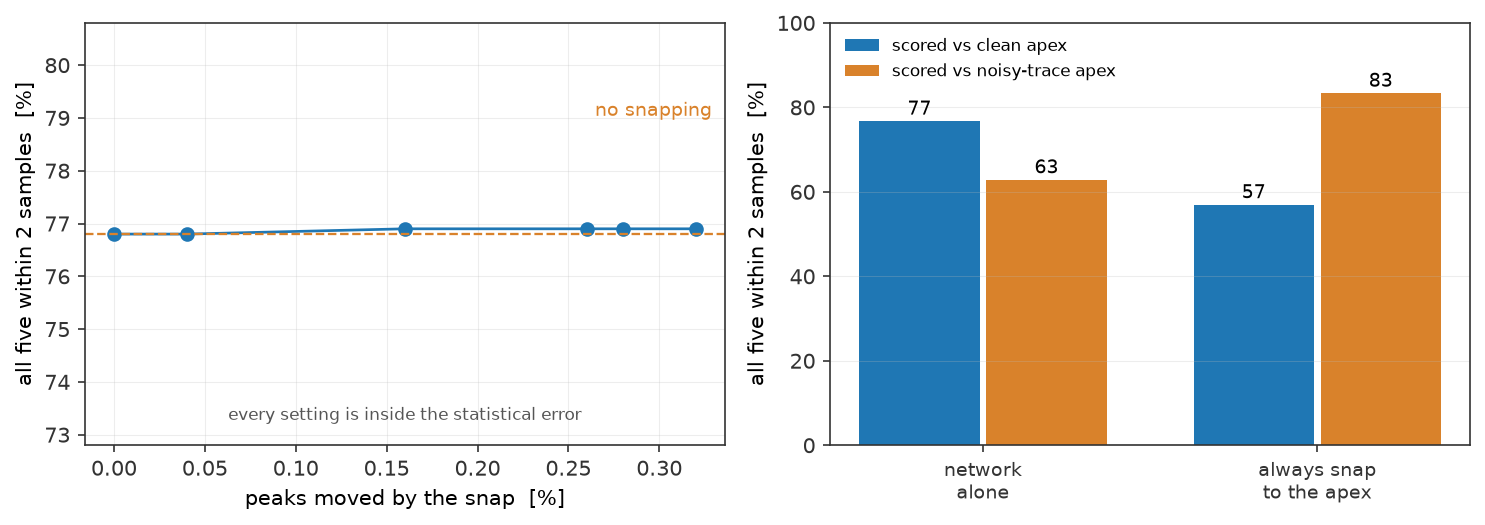
\includegraphics[width=0.95\textwidth]{toy/snap.png}
  \caption{Left: all-five-within-2 against the fraction of positions moved by the snap. Right: network
  alone and always-snap, scored against the clean apex and against the noisy-trace apex.}
  \label{fig:snap}
\end{figure}

\subsection{A two-stage hybrid, and why I dropped it}
I also tried scanning the trace for local maxima and letting a second-stage classifier assign candidates
to landmarks. Table~\ref{tab:hybrid} and Figure~\ref{fig:methods} compare it with the network alone. With
the network's own maxima added to the candidate list, the true landmark is among the candidates on 1000
of 1000 traces, and the network's answer breaks the time ordering on 1 of 1000 traces, so neither recall
nor ordering is the limitation. The second-stage ranker is a worse judge than the network output it
reads; I kept it as a switch, not the default.

\begin{table}[!htbp]
  \centering\small
  \caption{Hybrid variants on the same 1000 held-out traces; the ranker was trained on 2000 separate
  ones (\texttt{outputs/ablation.json}).}
  \label{tab:hybrid}
  \begin{tabular}{@{}lcc@{}}
    \toprule
    method & all five within 2 samples & any landmark $>15$ samples off \\
    \midrule
    network alone & 76.8\% & 2.0\% \\
    scan + ranker, ordered decode & 71.2\% & 2.1\% \\
    scan + ranker, plain decode & 71.4\% & 2.1\% \\
    scan + ranker, greedy & 71.2\% & 2.4\% \\
    \bottomrule
  \end{tabular}
\end{table}

\begin{figure}[!htbp]
  \centering
  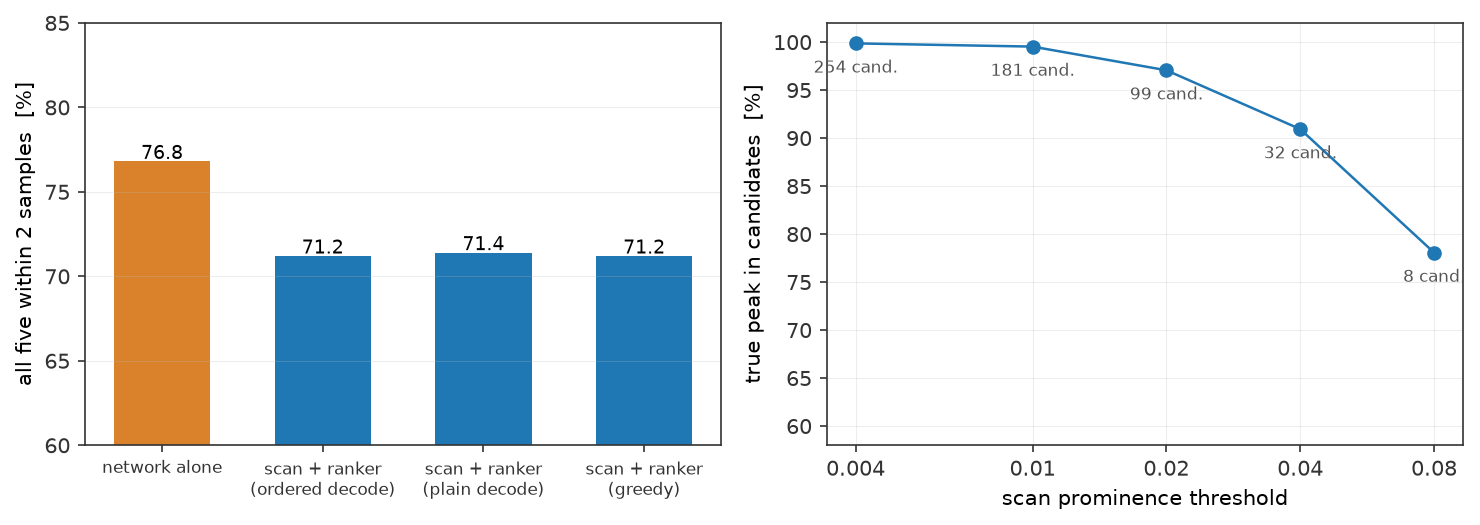
\includegraphics[width=0.95\textwidth]{toy/methods.png}
  \caption{Left: all five within 2 samples for each method. Right: how often the true landmark is among
  the scanned candidates, against the scan threshold; labels give candidates per trace.}
  \label{fig:methods}
\end{figure}

Other variants that did not beat the base model on toys: up-weighting the P0 channel in the loss, labels
on the rising edge instead of the apex (replaced by apex labels), and changes to target width, epoch
count and decoder.

%% ------------------------------------------------------------
\section{Real data}
\label{sec:data}

\subsection{The archive}
The tester archive holds one YAML result file per run and LeCroy \texttt{.trc} waveform files per shot. I
used only runs of the four-peak test (\texttt{expected\_peaks = 4}) whose C4 trace is in the archive:
\NShots\ shots in \NRuns\ runs, at input voltages \Vins. Each result file also records, per shot, what the
existing finder reported: label, time and height of each peak. The finder reported all four peaks on
\NGood\ shots and three on \NFail\ shots, all of them in \NFailRuns\ runs. I treated the archive as
untrusted input: extracted without owner or permission bits, YAML read with a safe loader only, nothing in
it executed.

\subsection{Reading the traces}
I read the \texttt{.trc} files with a short reader of my own (\texttt{src/trc.py}): value $=$ gain
$\times$ raw $-$ offset, time of sample $i$ $=$ horizontal offset $+\, i \times$ interval. Each trace has
250\,001 samples at 200\,ns. As a check, the current at the time the finder reports for a peak equals the
height it reports; so the finder reports the highest raw sample of each peak, not a smoothed apex.

\subsection{Binning}
I average each trace into bins of 50 samples (10\us), giving 5000 bins from $-5$ to 45\,ms after the
trigger, and pad to 5120 bins by holding the last value, so that the length divides by $2^L$ for the
U-Net. A landmark position is then a bin index, with fractional bins allowed in the labels.
Figure~\ref{fig:trace} shows one shot.

\begin{figure}[!htbp]
  \centering
  \includegraphics[width=0.95\textwidth]{real/trace.png}
  \caption{One held-out shot. Top: the full binned trace, with P0 marked and the region of P1--P4 shaded.
  Bottom: that region, with the existing finder's peaks (red $\times$) and the network's (blue $\circ$).}
  \label{fig:trace}
\end{figure}

\subsection{Labels}
\begin{itemize}
  \item \textbf{P0} is not reported by the finder. I label it by rule: the highest bin between $-5$ and
        $+3$\,ms.
  \item \textbf{P1--P4} are the finder's times for A1, B1, A2, B2, converted to bin index. Only shots where
        the finder reported all four are used for training.
\end{itemize}
The network is therefore trained to reproduce the existing finder, and on clean shots ``error'' below
means disagreement with the finder, not distance from a true position.

\subsection{Split by run}
Shots inside one run are close copies of each other, so I split by run, never by shot. The \NFailRuns\
runs that contain finder failures are held out entirely as a hard set (\NHard\ shots: \NFail\ failures
and \NHardClean\ clean shots). Of the remaining runs, 20\% chosen at random (seed 0) are the held-out set
for all numbers in Section~\ref{sec:results}: \NVal\ shots in \NValRuns\ runs. Training uses \NTrain\ shots
in \NTrainRuns\ runs.

%% ------------------------------------------------------------
\section{Training on real traces}
\label{sec:training}

Training uses AdamW (learning rate $10^{-3}$, weight decay $10^{-4}$) with a one-cycle schedule, batch
32, for \Epochs\ epochs, and the binary cross-entropy of Section~\ref{sec:method} with $\sigma =
\SigmaBins$ bins. Each training batch is augmented: a random shift of up to $\pm300$ bins (3\,ms), with
the labels moved along and the vacated end held at the edge value; a gain between 0.8 and 1.2; and added
Gaussian noise with a standard deviation drawn between 0 and 0.005 (in normalised units). The report
model trains in \WallUnet\,min on one RTX 4070. Figure~\ref{fig:training} shows the training loss and the
held-out agreement per epoch for three of the models of Section~\ref{sec:sweep}.

Repeated training with the same seed on the GPU does not reproduce bit for bit, so I compare
configurations across seeds rather than single runs (Section~\ref{sec:sweep}).

\begin{figure}[!htbp]
  \centering
  \includegraphics[width=0.95\textwidth]{real/training.png}
  \caption{Left: training loss per epoch. Right: held-out shots with all five landmarks within 0.02\,ms of
  their labels (argmax read-out). U-Net 16/3 (\texttt{u16}), U-Net 32/4 (\texttt{u32l4}, the report model)
  and transformer $256\times4$ (\texttt{t256x4}); seed 0.}
  \label{fig:training}
\end{figure}

%% ------------------------------------------------------------
\section{Results against the existing finder}
\label{sec:results}

All numbers in this section are on the \NVal\ held-out shots from \NValRuns\ runs never used in training,
for the U-Net 32/4 (seed 0) and, for comparison, the transformer ($d=128$, 4 layers, \ParamsTrans\,M
parameters), both with argmax read-out.

\begin{table}[!htbp]
  \centering\small
  \caption{Agreement with the existing finder on A1, B1, A2, B2, held-out runs.}
  \label{tab:summary}
  \begin{tabular}{@{}lccccc@{}}
    \toprule
    model & median $|\Delta t|$ [\textmu s] & all four $\le 0.02$\,ms & $\le 0.05$\,ms & $\le 0.1$\,ms
      & any $>1$\,ms \\
    \midrule
    U-Net 32/4 & \MedUnet & \TwoUnet\% & \FiveUnet\% & \TenUnet\% & \GrossUnet\% \\
    Transformer & \MedTrans & \TwoTrans\% & \FiveTrans\% & \TenTrans\% & \GrossTrans\% \\
    \bottomrule
  \end{tabular}
\end{table}

The network reads positions on a 10\us\ grid, while the finder uses the raw 200\,ns samples; differences
below about 5\us\ are the grid, not disagreement. Figure~\ref{fig:residuals} shows the signed
differences per peak and the fraction of shots with all four within a given tolerance.
Table~\ref{tab:perpeak} gives the same per landmark, including P0 against its rule label, and with the
sub-bin read-out.

\begin{figure}[!htbp]
  \centering
  \includegraphics[width=\textwidth]{real/residuals.png}
  \caption{Held-out shots. Four left panels: network minus finder per peak, U-Net 32/4, clipped at
  $\pm60$\us, log scale. Right: fraction of shots with all four within a tolerance, for both models; the
  dotted line is one 10\us\ bin.}
  \label{fig:residuals}
\end{figure}

\begin{table}[!htbp]
  \centering\small
  \caption{Per-landmark agreement with the training labels on held-out shots (P0 against its rule label,
  P1--P4 against the finder). Columns: median $|\Delta t|$ in \textmu s, then the percentage within
  0.02, 0.05 and 0.1\,ms, and beyond 1\,ms.}
  \label{tab:perpeak}
  \begin{tabular}{@{}llrrrrr@{}}
    \toprule
    model, read-out & landmark & median & $\le0.02$ & $\le0.05$ & $\le0.1$ & $>1$ \\
    \midrule
    \csname @@input\endcsname ../plots/real/perpeak_table.tex 
    \bottomrule
  \end{tabular}
\end{table}

\subsection{Shot-to-shot repeatability}
A comparison that needs no labels: within one run at one input voltage the shots should give nearly the
same times. For each such group with at least 5 held-out shots (\RepGroups\ groups) I compute the standard
deviation of each peak's time over the group, for the finder and for the network
(Figure~\ref{fig:repeat}). Median spread, finder against network: A1 \RepFAone\ vs \RepMAone\us, B1
\RepFBone\ vs \RepMBone\us, A2 \RepFAtwo\ vs \RepMAtwo\us, B2 \RepFBtwo\ vs \RepMBtwo\us. The network's
10\us\ grid limits how small its spread can look.

\begin{figure}[!htbp]
  \centering
  \includegraphics[width=\textwidth]{real/repeatability.png}
  \caption{Each point is one run at one voltage: standard deviation of the reported time over its shots,
  finder against network (U-Net 32/4). Below the line, the network is more repeatable.}
  \label{fig:repeat}
\end{figure}

\subsection{Example shots}
Figure~\ref{fig:clean} shows four held-out shots drawn at random, with both finders' peaks.

\begin{figure}[!htbp]
  \centering
  \includegraphics[width=0.95\textwidth]{real/clean_shots.png}
  \caption{Four held-out shots, 15--27\,ms after the trigger. Red $\times$: existing finder, with its labels.
  Blue $\circ$: network.}
  \label{fig:clean}
\end{figure}

%% ------------------------------------------------------------
\section{Shots where the existing finder failed}
\label{sec:failures}

On \NFail\ shots, all in \NFailRuns\ runs, the finder reported three peaks, labelled \FailLabels, instead
of A1, B1, A2, B2. These runs were never used in training. The network places all five landmarks on every
one of them; Figure~\ref{fig:fail} shows six. There is no reference for A1 on these shots, so this part
is a visual and consistency check, not a measured error. On the \NHardClean\ clean shots of the same runs,
all five landmarks lie within 0.02\,ms of their labels on \HardTwo\% and within 0.1\,ms on \HardTen\%.

\begin{figure}[!htbp]
  \centering
  \includegraphics[width=0.95\textwidth]{real/failure_shots.png}
  \caption{Six of the \NFail\ shots where the existing finder reported three peaks. Red $\times$: finder,
  with its labels. Blue $\circ$: network.}
  \label{fig:fail}
\end{figure}

\paragraph{Confidence.}
Figure~\ref{fig:conf} shows the per-landmark confidence on held-out shots, and the A1 confidence on clean
shots against the finder's failures. The median A1 confidence is \ConfClean\ on clean held-out shots and
\ConfFail\ on the failure shots, with the lowest failure shot at \ConfFailMin. The failure shots do not
stand out in confidence.

\begin{figure}[!htbp]
  \centering
  \includegraphics[width=0.95\textwidth]{real/confidence.png}
  \caption{Left: confidence per landmark, held-out clean shots, log scale. Right: A1 confidence, held-out
  clean shots against the finder's failure shots (normalised).}
  \label{fig:conf}
\end{figure}

%% ------------------------------------------------------------
\section{Model size and training seed}
\label{sec:sweep}

To see whether a larger network agrees better, I trained five U-Nets and two transformers on the same
split for the same \Epochs\ epochs, and repeated U-Net 16/3 and U-Net 32/4 with two more seeds (Table~\ref{tab:sweep}, Figure~\ref{fig:sweep}). These numbers include P0 and are against the
training labels.

\begin{table}[!htbp]
  \centering\small
  \caption{Model-size sweep on the held-out shots. Where a model has more than one seed, a cell shows the
  mean and, in brackets, the lowest and highest seed. ``Sub-bin'' is the parabola read-out of
  Section~\ref{sec:method}.}
  \label{tab:sweep}
  \footnotesize\setlength{\tabcolsep}{2.5pt}
  \begin{tabular}{@{}lrrrrrrr@{}}
    \toprule
    model & params [M] & seeds & train [min] & \multicolumn{2}{c}{all five, argmax [\%]} & sub-bin [\%]
      & $>1$\,ms [\%] \\
    \cmidrule(lr){5-6}
    & & & & $\le0.02$\,ms & $\le0.05$\,ms & $\le0.02$\,ms & \\
    \midrule
    \csname @@input\endcsname ../plots/real/sweep_table.tex 
    \bottomrule
  \end{tabular}
\end{table}

\begin{figure}[!htbp]
  \centering
  \includegraphics[width=0.6\textwidth]{real/sweep.png}
  \caption{All five within 0.02\,ms (sub-bin read-out) against parameter count; one point per training
  run.}
  \label{fig:sweep}
\end{figure}

No larger network clearly beats the smallest one at seed 0, and the U-Nets lie close together while the
transformers lie lower. Across three seeds, however, the 16/3 U-Net spreads widely while the 32/4 U-Net
stays within a narrow band (Table~\ref{tab:sweep}). I therefore use the 32/4 U-Net, seed 0, as the report
model in Sections~\ref{sec:results} and~\ref{sec:failures}.

%% ------------------------------------------------------------
\section{Status and open items}
\label{sec:status}

\paragraph{Unsigned steps.} Four steps of the real-data chain have not been signed off, and every number
from real data in this note depends on them: the dataset build and the P0 rule; the run-level split;
network training; and the peak read-out (argmax per channel on 10\us\ bins, and the sub-bin read-out).

\paragraph{Limits of this comparison.}
\begin{itemize}
  \item On clean shots the labels are the existing finder's own times, so agreement measures how well the
        network reproduces the finder, not how close either is to a true position.
  \item The P0 label is a rule (highest bin between $-5$ and $+3$\,ms), and the network reproduces it.
  \item On the failure shots there is no reference for A1.
  \item The network's positions are on a 10\us\ grid; the finder's are on the 200\,ns samples.
  \item The failure shots come from only \NFailRuns\ runs.
\end{itemize}

\paragraph{Next.}
\begin{itemize}
  \item Write the algorithm description of the four real-data steps and go through sign-off.
  \item Obtain independent labels on the hard cases, in particular on shots the present finder gets
        wrong, to measure the network's error there rather than check it visually.
\end{itemize}

%% ------------------------------------------------------------
\clearpage
\appendix
\section{Reproducing this note}
All commands run from the repository root; \texttt{\$ENV} is the Python environment. The full procedure,
with expected outputs, is in \texttt{docs/RUNBOOK\_vfe\_peak\_ml-DETAIL.md}.

\begin{small}
\begin{verbatim}
# toys
micromamba run -n $ENV python -m src.train
micromamba run -n $ENV python -m src.hybrid
micromamba run -n $ENV python -m diagnostics.hybrid_ablation
micromamba run -n $ENV python -m diagnostics.refine_sweep
micromamba run -n $ENV python -m diagnostics.refine_gated
micromamba run -n $ENV python -m diagnostics.apex_ambiguity

# real data
micromamba run -n $ENV python -m src.real_data \
    <yaml_dir> ~/Downloads/results.tar <members.txt> data
micromamba run -n $ENV python -m src.train_real --arch unet \
    --base 32 --levels 4 --out outputs/real/sweep/u32l4
micromamba run -n $ENV python -m src.train_real --arch transformer \
    --out outputs/real/transformer
# model-size sweep and extra seeds: runbook step 16

# this note
micromamba run -n $ENV python -m writeup.make_figures
cd writeup/src && pdflatex -output-directory=../outputs vfe_peak_ml_writeup.tex
\end{verbatim}
\end{small}

\end{document}
